L’algoritmo di Canny è uno dei più popolari algoritmi di riconoscimento dei contorni. L’algoritmo punta a trovare il maggior numero di contorni nell’immagine vicini ai contorni reali evitando di marcare più volte lo stesso contorno ed evitando di provocare falsi riconoscimenti.

E’ un algoritmo multi-stadio che si articola in 4 fasi:
\begin{enumerate}
  \item Riduzione del rumore
  \item Ricerca del gradiente della luminosità di un'immagine
  \item Soppressione dei non-massimi
  \item Individuazione dei contorni mediante sogliatura con isteresi
\end{enumerate}

Nella libreria OpenCV dell’algoritmo di Canny viene implementato dalla funzione \texttt{cv2.Canny}.

\begin{minted}
  [
    xleftmargin=\parindent,
    framesep=2mm,
    baselinestretch=1.2,  
    fontsize=\footnotesize,
    linenos,
    breaklines
  ]
  {python}
  
  canny = cv2.Canny(thresh, config.HOUGH_IRIS.getint(
   'CANNY_TH1'), config.HOUGH_IRIS.getint('CANNY_TH2'))   
\end{minted}

La funzione in automatico applica tutti e 4 gli stadi precedentemente citati, gli unici input obbligatori sono: l’immagine, che deve essere necessariamente in grayscale (single-channel), e due valori di soglia (chiamati threshold) per la procedura di isteresi. 

Nell'elaborato il Canny Edge viene utilizzato esclusivamente nella funzione di riconoscimento dell’iride, in particolare lo si applica all’immagine binaria (bianca e nera) ottenuta dalla precedente operazione di thresholding con i due parametri di soglia settati a 150 e 200 (\texttt{CANNY\_TH1} e \texttt{CANNY\_TH2}) . Si è scelto di utilizzarlo solo per la parte di riconoscimento dell’iride  in quanto il threshold di per sé non bastava a portare una buona accuratezza nel riconoscimento della circonferenza. Infatti, a differenza della pupilla che ha tutti i valori di pixel vicino al nero, per la parte dell’iride non esiste un valore di soglia che sia in grado di evidenziare la sola  area di iride in quanto ci possono essere delle parti dell’occhio, diversi dall’iride, con valori dei pixel inferiori alla soglia che vengono categorizzati come nero. La seguente immagine evidenzia questo problema, si nota infatti come, a differenza della pupilla, l’area di interesse dell’iride non venga perfettamente delineata.

\begin{figure}[h]
  \centering
  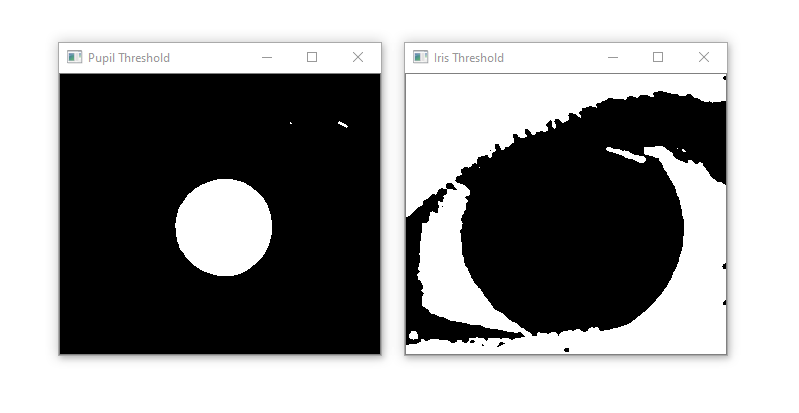
\includegraphics[width=1.0\textwidth]{canny_threshold.png}
  \caption{Confronto tra il risultato del threshold per iride e pupilla}
\end{figure}

Si è quindi ritenuto necessario applicare l’algoritmo di Canny al solo riconoscimento dell’iride in modo da definire il più possibile l’area di interesse, mentre per la pupilla non è risultato necessario applicare ulteriori trasformazioni.

\begin{figure}[h]
  \centering
  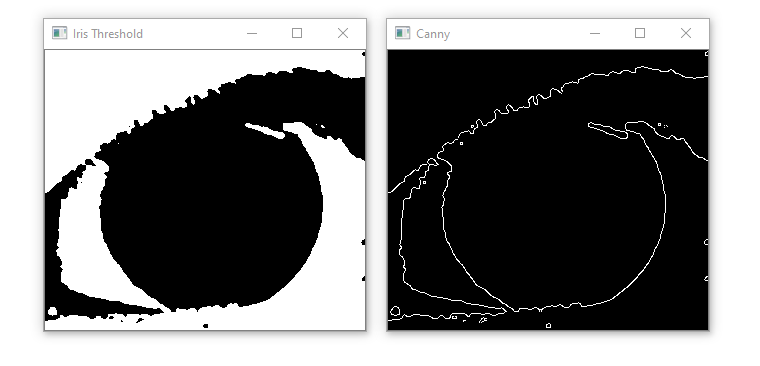
\includegraphics[width=1.0\textwidth]{canny_edge.png}
  \caption{Applicazione del Canny Edge Detector in successione al treshold}
\end{figure}

Il risultato ottenuto dal Canny Edge è quindi un’immagine in cui gran parte dei contorni dell’iride è ben definito e ciò risulta essere molto utile per il passo successivo ovvero l’identificazione di cerchi nell’immagine. Il Canny di fatto fornisce all’algoritmo di riconoscimento  già una buona parte della circonferenza dell’iride e di conseguenza risulterà anche più semplice ed accurato il riconoscimento della circonferenza completa.
